%%%%%%%%%%%%%%%%%%%%%%%%%%%%%%%%%%%%%%%%%%%%%%%%%%%%%%%%%%%%%%%%%%%%
%%%%%%%%%%%%%%%%%%%%%%%%%%%%%%%%%%%%%%%%%%%%%%%%%%%%%%%%%%%%%%%%%%%%
%%                                                                %%
%% An example for writting your thesis using LaTeX                %%
%% Original version by Luis Costa,  changes by Perttu Puska       %%
%% Support for Swedish added 15092014                             %%
%%                                                                %%
%% This example consists of the files                             %%
%%         thesistemplate.tex (versio 2.01)                       %%
%%         opinnaytepohja.tex (versio 2.01) (for text in Finnish) %%
%%         aaltothesis.cls (versio 2.01)                          %%
%%         kuva1.eps                                              %%
%%         kuva2.eps                                              %%
%%         kuva1.pdf                                              %%
%%         kuva2.pdf                                              %%
%%                                                                %%
%%                                                                %%
%% Typeset either with                                            %%
%% latex:                                                         %%
%%             $ latex opinnaytepohja                             %%
%%             $ latex opinnaytepohja                             %%
%%                                                                %%
%%   Result is the file opinnayte.dvi, which                      %%
%%   is converted to ps format as follows:                        %%
%%                                                                %%
%%             $ dvips opinnaytepohja -o                          %%
%%                                                                %%
%%   and then to pdf as follows:                                  %%
%%                                                                %%
%%             $ ps2pdf opinnaytepohja.ps                         %%
%%                                                                %%
%% Or                                                             %%
%% pdflatex:                                                      %%
%%             $ pdflatex opinnaytepohja                          %%
%%             $ pdflatex opinnaytepohja                          %%
%%                                                                %%
%%   Result is the file opinnaytepohja.pdf                        %%
%%                                                                %%
%% Explanatory comments in this example begin with                %%
%% the characters %%, and changes that the user can make          %%
%% with the character %                                           %%
%%                                                                %%
%%%%%%%%%%%%%%%%%%%%%%%%%%%%%%%%%%%%%%%%%%%%%%%%%%%%%%%%%%%%%%%%%%%%
%%%%%%%%%%%%%%%%%%%%%%%%%%%%%%%%%%%%%%%%%%%%%%%%%%%%%%%%%%%%%%%%%%%%

\documentclass[english,12pt,a4paper,pdftex,eng,utf8]{aaltothesis}

%% To the \documentclass above
%% specify your school: arts, biz, chem, elec, eng, sci
%% specify the character encoding scheme used by your editor: utf8, latin1

\usepackage{graphicx}

%% Use this if you write hard core mathematics, these are usually needed
\usepackage{amsfonts,amssymb,amsbsy}

\usepackage{color}

\definecolor{xkcd_blue}{RGB}{3,67,223} % https://xkcd.com/color/rgb/

%% Use this if you want to get links and nice output. Works well with pdflatex.
\usepackage{hyperref}
\hypersetup{
  pdfpagemode=UseNone,
  pdfstartview=FitH,
  colorlinks=true,
  urlcolor=xkcd_blue,
  linkcolor=black,
  citecolor=black,
  pdftitle=A Model for Selecting Software Tools for Fluid Power Systems,
  pdfauthor=Fletcher Porter,
  pdfkeywords={
    Mechatronics,Tooling,Automation,Instrumentation,Tech Stack
  }
}

\usepackage[ddmmyyyy]{datetime}
\renewcommand{\dateseparator}{.}

\usepackage{siunitx}
\usepackage{gensymb}
\usepackage{svg}
\usepackage{lipsum}  % for placeholder text

%% All that is printed on paper starts here
\begin{document}

%% Change the school field to specify your school if the automatically 
%% set name is wrong
% \university{aalto-yliopisto}
% \university{aalto University}
% \school{Sähkötekniikan korkeakoulu}
% \school{School of Electrical Engineering}

%% Only for B.Sc. thesis: Choose your degree programme. 
%\degreeprogram{Electronics and electrical engineering}
%%

%% ONLY FOR M.Sc. AND LICENTIATE THESIS: Specify your department,
%% professorship and professorship code. 
%%
\department{Department of Mechanical Engineering}
\professorship{Mechatronics}
%%

%% Valitse yksi näistä kolmesta
%%
%% Choose one of these:
%\univdegree{BSc}
\univdegree{MSc}
%\univdegree{Lic}

%% Your own name (should be self explanatory...)
\author{Fletcher Porter}

%% Your thesis title comes here and again before a possible abstract in
%% Finnish or Swedish . If the title is very long and latex does an
%% unsatisfactory job of breaking the lines, you will have to force a
%% linebreak with the \\ control character. 
%% Do not hyphenate titles.
%% 
\thesistitle{A Model for Selecting Software Tools for Fluid Power Systems}

\place{Espoo}

%% For B.Sc. thesis use the date when you present your thesis. 
%% 
%% Kandidaatintyön päivämäärä on sen esityspäivämäärä! 
\date{\today}

%% B.Sc. or M.Sc. thesis supervisor 
%% Note the "\" after the comma. This forces the following space to be 
%% a normal interword space, not the space that starts a new sentence. 
%% This is done because the fullstop isn't the end of the sentence that
%% should be followed by a slightly longer space but is to be followed
%% by a regular space.
%%
\supervisor{Prof.\ Jari Vepsäläinen}

%% B.Sc. or M.Sc. thesis advisors(s). You can give upto two advisors in
%% this template. Check with your supervisor how many official advisors
%% you can have.
%%
\advisor{D.Sc. (tech) Olof Colonius}

%% Aalto logo: syntax:
%% \uselogo{aaltoRed|aaltoBlue|aaltoYellow|aaltoGray|aaltoGrayScale}{?|!|''}
%%
%% Logo language is set to be the same as the document language.
%% Logon kieli on sama kuin dokumentin kieli
%%
\uselogo{aaltoRed}{''}

%% Create the coverpage
%%
\makecoverpage


%% Note that when writting your master's thesis in English, place
%% the English abstract first followed by the possible Finnish abstract

%% English abstract.
%% All the information required in the abstract (your name, thesis title, etc.)
%% is used as specified above.
%% Specify keywords
%%
%% Kaikki tiivistelmässä tarvittava tieto (nimesi, työnnimi, jne.) käytetään
%% niin kuin se on yllä määritelty.
%% Avainsanat
%%
\keywords{Mechatronics,Tooling,Automation,Instrumentation,Tech Stack}
%% Abstract text
\begin{abstractpage}[english]
Mechatronic systems can be enormously complex.  Possibly the chiefest complexity is in their software components due the the deep knowledge required for effective development, the need to interface with myriad heterogeneous components, and the opacity of its operation.  I'll be speaking about alleviating these issues by introducing a novel theory for specifying and discussing the need for software tools and then a case study in applying this theory in the development of a Stewart Platform used as a driving simulator platform. 
\end{abstractpage}

%% Force a new page so that the possible English abstract starts on a new page
%%
%% Pakotetaan uusi sivu varmuuden vuoksi, jotta 
%% mahdollinen suomenkielinen ja englanninkielinen tiivistelmä
%% eivät tule vahingossakaan samalle sivulle
\newpage

%% Preface
%%
%% Esipuhe 
\mysection{Preface}
%\mysection{Esipuhe}
I'd like to thank my teachers for making me wise, my family and friends for making me me, and the wind for guiding me in interesting directions. \\

\vspace{5cm}
Otaniemi, \today

\vspace{5mm}
{\hfill Fletcher Porter \hspace{1cm}}

%% Force new page after preface
%%
%% Pakotetaan varmuuden vuoksi esipuheen jälkeinen osa
%% alkamaan uudelta sivulta
\newpage


%% Table of contents. 
\thesistableofcontents


%% Symbols and abbreviations
\mysection{Symbols and abbreviations}

\subsection*{Symbols}

\begin{tabular}{ll}
$\mathbf{B}$  & magnetic flux density  \\
$c$              & speed of light in vacuum $\approx 3\times10^8$ [m/s]\\
$\omega_{\mathrm{D}}$    & Debye frequency \\
$\omega_{\mathrm{latt}}$ & average phonon frequency of lattice \\
$\uparrow$       & electron spin direction up\\
$\downarrow$     & electron spin direction down
\end{tabular}

\subsection*{Operators}

\begin{tabular}{ll}
$\nabla \times \mathbf{A}$              & curl of vectorin $\mathbf{A}$\\
$\displaystyle\frac{\mbox{d}}{\mbox{d} t}$ & derivative with respect to 
variable $t$\\[3mm]
$\displaystyle\frac{\partial}{\partial t}$  & partial derivative with respect 
to variable $t$ \\[3mm]
$\sum_i $                       & sum over index $i$\\
$\mathbf{A} \cdot \mathbf{B}$    & dot product of vectors $\mathbf{A}$ and 
$\mathbf{B}$
\end{tabular}

\subsection*{Abbreviations}

\begin{tabular}{ll}
  IT & Information Technology \\
  HTML & Hyper Text Markup Language \\
  SQL & Structured Query Language \\
  CAN & Controller Area Network \\
  OSI & Open Systems Interconnection \\
  DDH & Directy-Drive Hydraulics \\
  EHA & Electro-Hydraulic Actuator \\
  ECU & Electronic Control Unit \\
  DAQ & Data Acquisition \\
  IO & Input/Output \\
  PLC & Programmable Logic Controller \\
  TCP & Transmission Control Protocol \\
  IP & Internet Protocol \\
  UDP & User Datagram Protocol \\
  IDE & Integrated Development Environment \\
\end{tabular}


%% Tweaks the page numbering to meet the requirement of the thesis format:
%% Begin the pagenumbering in Arabian numerals (and leave the first page
%% of the text body empty, see \thispagestyle{empty} below).
%% Additionally, force the actual text to begin on a new page with the 
%% \clearpage command.
%% \clearpage is similar to \newpage, but it also flushes the floats (figures
%% and tables).
%% There is no need to change these
%%
\cleardoublepage
\storeinipagenumber
\pagenumbering{arabic}
\setcounter{page}{1}


\section{Introduction}

%% Leave first page empty
\thispagestyle{empty}

Mechatronic systems are enormously complex.  The name {\it mechatronics\/} betrays that it involves work with mechanics and electronics, but as well a mechatronics engineer needs to also be a practitioner of software, hydraulics, and pneumatics.  In the research environments where typically mechatronics engineers are found, they also need the practical knowledge to implement their designs, like how to assemble a circuit that gets a signal from A to B, or how do you merge software contributions from multiple collaborators.

To create all of this from first principals is such a massive, untenable task.  Fortunately, the engineers of the past have left behind knowledge and tools to overcome these kinds of challenges.  However, even the most tenacious researcher struggles to find and grasp all of this knowledge.  It would ease the burden to have a structured method for describing these tools.  The work of this thesis will be to create just that---a novel, structured categorization of tools used in mechatronics, which I'll call a {\it Mechatronic Tech Stack}.

\subsection{Motivation}

\lipsum[1-3]

\subsection{Objective}

\lipsum[1-3]

\subsection{Scope}

\lipsum[1-3]

\subsection{Methodology}

\lipsum[1-3]

\subsection{Thesis Structure}

\lipsum[1]

\clearpage


\section{Theory}

This section constructs the backbone of this thesis, namely the novel theory of a mechatronic tech stack.  First, there will be a review of tech stacks and {\it abstraction layers\/} as they've been applied in the IT sector.  Then there will be a proposal of a mechatronic tech stack determined by a standards-based set of principals.

\subsection{Technology Stacks in the IT Sector}

A concept of a tech stack, alternately called a solution stack or a software stack, is to enumerate the tasks done by a kind of software application and to suggest tools for those tasks~\cite{PranamStack2017}.  More specifically, it defines a set of abstraction layers; each layer abstractly describes a type of task and contains within it the set of software tools that complete that task.  The intention is to take the difficult task of tool selection and provide a structure through which practitioners can think about the functions and tooling needs of their application, freeing mental energy to critically assess which tools would be best for their technical and personnel needs.

\subsubsection{The Web Stack}

A ubiquitous example of a tech stack in IT is the {\it web stack}, used for developing websites and related pieces of software.  The tasks that websites must perform, as suggested by this stack, are to present an interface to a user through a web browser (the {\it front end\/}), to conduct some business logic like creating a customized page for the user (the {\it back end\/}), to perform network communication (the {\it server\/}), and to store and dispatch data (the {\it database\/})~\cite{PranamStack2017}.  This doesn't describe all websites---many don't have databases or any real back-end logic, but it describes at least a superset of the functionality of most websites.

Tools in each of these layers are myriad and to highlight that, proceeding is a list of a small sample.  You can also observe this in figure~\ref{fig:web_stack}  Front-end tools like jQuery~\cite{jQuery} have been proven from many years of use, React~\cite{React} is extrodinarily powerful and can be used in non-web contexts as well, and even plain HTML without an additional framework can be good on account of its simplicity.  Backend tools can allow a developer to select their favorite programming language, or one that is specialized for web backends, or even JavaScript like the front end uses.  Servers are often integrated into the back-end framework, but if not, specialized servers like Apache~\cite{ApacheServer} or nginx~\cite{nginx} are popular.  Databases are dominated by reliable and proven relational, SQL-based offerings, but alternatives like the confusingly named NoSQL or Redis~\cite{redis} have become popular in the past years on account of their performance and scalability.

\begin{figure}[h]
  \centering
  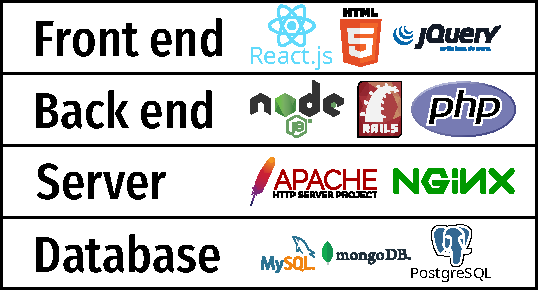
\includegraphics[width=0.5\textwidth]{assets/web_stack}
  \caption{The web stack is like 4 bins of tools, here illustrated as boxes with the logos of common tools within them.}\label{fig:web_stack}
\end{figure}

In discussing the web stack, it's also useful to think about a particular set of tools used for a single project, i.e.\ one tool from each layer.  Alternately, this can be thought of as the project's {\it cross section\/} of the web stack, or the the project's own stack.  There are several of these cross sections that are widely used, such as LAMP (Linux, Apache, MySQL, PHP) or MEAN (MongoDB, Express.js, Angular.js, Node.js)~\cite{PranamStack2017}.  Just as often, firms employ stacks tailored to their technical and personnel needs and often write about these decisions in blog posts, such as for recent changes to Microsoft Teams in~\cite{Singh2023}.

\subsubsection{OSI Network model}

Another example of a tech stack is the OSI Network model which abstractly describes network communication down to the lowest levels of physical signaling up to the highest levels of abstract behaviour~\cite{ISO7498-1}.  This model is frequently cited in mechatronic literature since many fieldbus protocols like CAN define their functionality in terms of this model.  This model is also interesting since its standard description (ISO~7498-1) also includes principal for creating layered models of a similar ilk.

The OSI model differs from the web stack in how the layers are used by practitioners.  Typically, instead of each layer being a bin to pick a tool from and where a tools must be picked from every layer which you want functionality, developers instead may decide at what depth into the model they begin their implementation and assume everything below that depth ``just works''.

To spare a moment for the details of the model, it consists of layered abstraction over physical communication media, as seen in figure~\ref{fig:osi_model}.  The lowest layer, Physical, concerns itself with the physical phenomena of communication.  In the case of CAN, this means voltage levels, terminating resistors, twisted pairs, grounding rules, and more.  The highest level, Application, provides network facilities without need for understanding {\it how\/} the network connection is made.  The Application layer includes, for example, identifying communication partners and negotiating security protocols.  Well-known protocols like HTTP, DNS, and FTP exist in the Application layer.  The intermediate layers basically provide increasing levels of abstraction over the physical layer, defining things like the structure of data packets, how to route messages, how to route them efficiently, and more.

\begin{figure}[h]
  \centering
  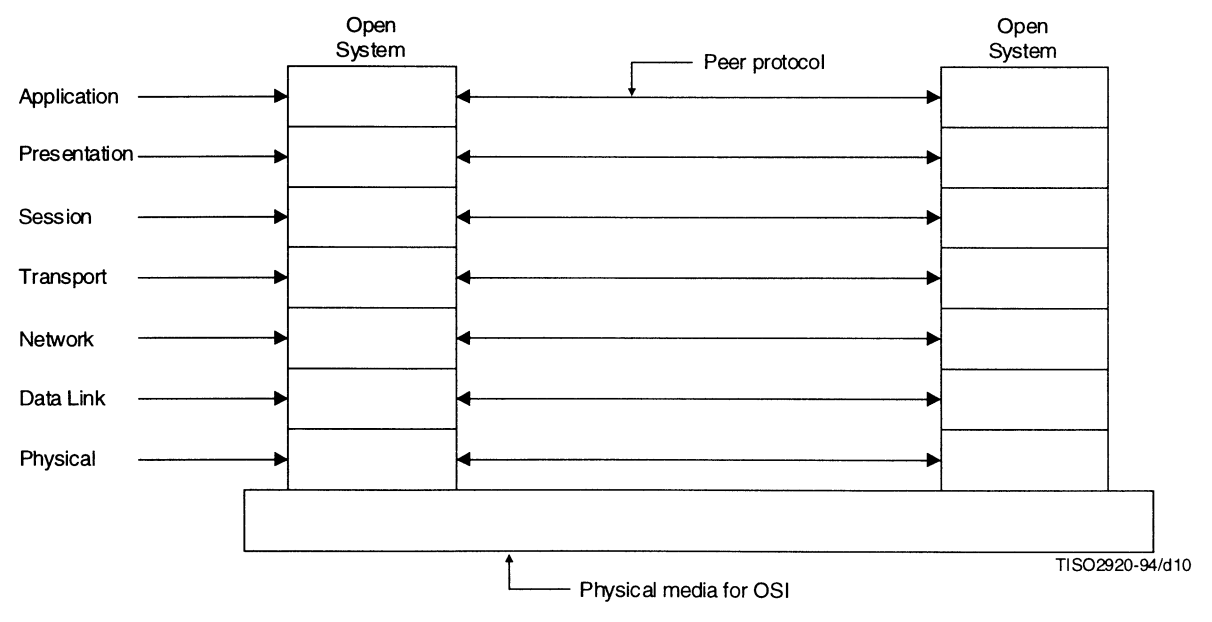
\includegraphics[width=0.6\textwidth]{assets/osi_model}
  \caption{The OSI model understands network communication to be a layer cake of abstractions over the physical communication media.  Taken from~\cite[§6.1.3]{ISO7498-1}.}\label{fig:osi_model}
\end{figure}

An interesting property of this layered abstraction architecture is that protocols which are defined in higher layers can often have the lower layers transparently replaced.  For instance, the internet protocol which we use every day is defined in the Network and Transport layers.  Typically the lower-level protocols used with IP are Ethernet and IEEE~802.11 (Wi-Fi).  However, with some implementation effort, other low-level protocols are available.  Lindgren et al.\ developed IP over CAN, wherein an internet network is extended over a CAN network~\cite{Lindgren2008}, something which was never imagined by implementors of CAN nor IP.\

\subsubsection{Principles for Identifying Abstraction Layers}

The OSI standard also includes the principals upon which its layers were designed~\cite[§6.2.1]{ISO7498-1}.  In summary, each layer should be a discrete, seperable item with a coherant function.  The interfaces between layers should be succinct and only interface with adjacent layers.  It suggests having fewer layers would ease explanation and implementation and it offers a test to aid in determining layer boundaries.  It also says that the layers should be motivated by experience.  Being a novel theory, experience will be the principal gain of future work, although case studies discussed later will provide somewhat in this dimension.  A layer should have a different level of abstraction in terms of {\it morphology}, {\it syntax}, and {\it semantics}.

This model of morphology, syntax, and semantics come from Bloomfieldian linguistics~\cite{Bloomfield1923}.  It's used to coerce natural languages into a structured form from which meaning can be gleaned.  Here, the standard authors are using it to glean structure and meaning from engineering systems.  To understand this model, take this line of C code.

\begin{verbatim}
printf("I have %u cows\n", num_cows);
\end{verbatim}

Morphology is concerned with the atomic elements of meaning.  In C code, this means short tokens of text (also called morphemes), here \verb|printf|, \verb|(|, \verb|"I have %u cows\n"|, \verb|,|, \verb|num_cows|, \verb|)|, and \verb|;|.  None of these can be cut in half and still carry meaning---\verb|pri| and \verb|ntf| doesn't make \verb|printf|.  But these atoms of meaning needn't just be text or language.  As will be discussed below, these atoms can be cables, connectors, computer hardware, or really anything that can have meaning when combined with other things.

When these morphemes are combined into phrases, that's syntax.  Syntax is the structure into which meaning is applied.  The \verb|printf| example is syntactically parsed by C compilers as in figure~\ref{fig:printf_syntax}.  The syntax tells that the postfix expression represented by the identifier \verb|printf| has the argument list of \verb|"I have %u cows\n"| (a string literal) and \verb|num_cows| (an identifier).  What any of these tokens mean is not the domain of syntax, but instead semantics.

\begin{figure}[h]
  \centering
  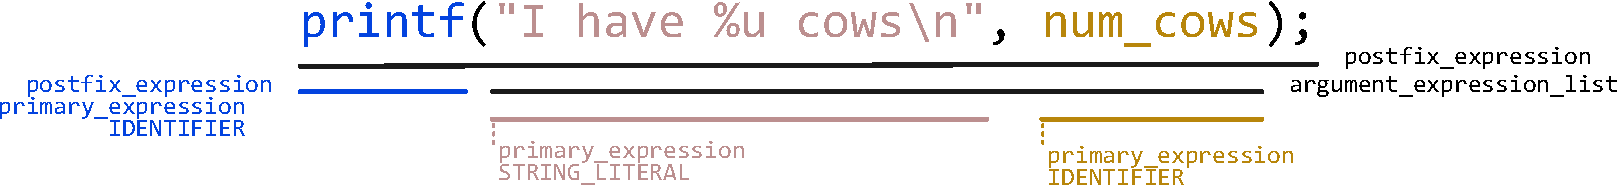
\includegraphics[width=0.8\textwidth]{assets/printf_syntax}
  \caption{The above printf example with syntax labeled according to K{\&}R C~\cite{Kernighan1978}}\label{fig:printf_syntax}
\end{figure}

To understand the semantics of \verb|printf|, you must read the documentation.  It will tell you that \verb|printf| means to convert and write output to the console under the control of a format string.  You'll also see that \verb|"I have %u cows\n"| is that format string, and \verb|num_cows| is an additional argument, presumably the number of cows the author has.  In fact, reading the documentation further, you'll learn that the format string itself has its own morphology, syntax, and semantics driving how formatted output is created.

Technology stacks, like the web stack or the OSI stack, create a structure for selecting tools for an application and abstractions for interfacing with other layers of the stack.  The OSI model also provides guidance on how to architect a layered model based, among other things, on creating layers with coherant morphology, syntax, and semantics.

In the next section, this knowledge will be applied to create a mechatronic tech stack with the properties of the web and OSI stacks.

\subsection{A Mechatronic Tech Stack}

Broadly speaking, mechatronic systems include mechanical systems, power-electronic systems, and digital control systems (neglecting mechanical governors and analog control circuits).  All of these could be considered under a theory of a mechatronic tech stack, but the present treatment will only consider the control systems.  More specifically, this stack will start just after any sensors or transducers, giving those items IO (input/output) hookups.

The layers will by identified by noting contrasts in morphology, syntax, and semantics thoughout the gamut of the control system.  Layer boundaries will become evident where differences in these aspects are dramatic.  I'll then describe the layers and the interfaces between them.

Morphology provides the strongest and most coarse distinctions in layers.  If the atoms that one component is made of are incompatible with another, they can't effectively be abstracted together.  The most obvious case is that those components that are made of literal atoms, i.e.\ hardware, must be considered separately from those that aren't physical, namely software.  Within hardware, a control engineer will concern themselves with the components of the computer which their control softwares run on (RAM, CPU, storage, etc.) and the physical connections between the computer components and the sensors and transducers, such as cables, connectors, contacts, and traces.  Making up the software is the instructions of the control program itself, but also supporting software like the operating system, runtime environments, and useful libraries.

Syntax is the structure of an idea.  It is a finer comb to discriminate layers.  Software generally is built as a linear sequence of instructions with branches and loops.  This describes the control engineer's perspective on their own control program, but supporting software like libraries are more abstract.  They're better thought of as a dependency.  A control program may depend on libraries A, B, and C, and those in turn depend on libraries D, E, F, and G.  These {\it middlewares\/} are better understood as a network of the softwares themselves and the dependency connections between them.  For hardware, its structure is its assemblage.  The computer components are connected to the motherboard, sensors and transducers are connected to a CAN bus, the temperature sensors communicate over I2C, etc.  Like middleware, hardware is the network of components and the connections between them, but the type of connection is also important.  A system with components on a CAN bus is going to be different than one with a USB bus, and different still from a system where all components communicate over a serial connection.

Semantic meaning reveals the most subtle distinctions in layers.  The control program is an expression of the business logic desired by the control engineer.  It is whatever control logic that is asked of the engineer.  Middleware begins where the controller ends, which is to say it is abstraction around the computer's function.  It attempts to save the engineer from difficult, tedious, or uninteresting implementation.  The middleware ends where the computer begins.  Computers are meaningful when they provide compelling output based on some input.  That is to say, when they compute.  How this computation occurs at the hardware level is determined by the computers {\it architecture}.  This defines what machine instructions do what, which hardware pins go where, and how it should all be connected.  IO is the hardware beyond the computer.  Its is the language of data transfer.  A sensor's pressure reading becomes a message to the computer.  The computer's actuation command becomes a message to the transducer.  This is handled by netowrk communication protocols, the domain of the OSI model.

This is enough to propose a mechatronic tech stack.  The mechatronic stack as outlined sits on top of signaling with sensors and transducers.  Those are interfaced by IO systems that connect to computer systems which run middleware upon which a control program depends.  This is illustrated as a stack diagram in figure~\ref{fig:mechatronic_tech_stack}.

\begin{figure}[h]
  \centering
  \includegraphics[width=0.5\textwidth]{assets/mechatronic_tech_stack}
  \caption{The mechatronic tech stack places high-level business logic at the top and low-level interfacing at the bottom.  This sits atop hardware intrumentation, where this theory placed its limit.}\label{fig:mechatronic_tech_stack}
\end{figure}

Between the layers are the interfaces that enable higher layers to take advantage to take advantage of the abstractions provided by lower layers.  The control layer, being the highest, provides no interface to further layers, but from the middleware layer it demands certain {\it application programming interfaces}, or APIs.  Each program in the middleware layer (generally) provides an API, so the control-middleware interface is the union of all of these APIs.  The needs of middleware are typically met by other middleware, but those that interface with the computer directly do so through architecture-defined machine code.  Then for the Computer-IO interface, the IO needs some hardware connection like pins broken out from the CPU, integral connection ports like for USB, serial, or RJ45 (Ethernet).  Finally, IO interfaces with sensors and transducers in the same way it does with computers, through hardware interfaces like terminal blocks or hookups to a fieldbus.

This model, like the web stack, provides a structure through which to think about tool selection.  The choice of using CAN- or serial-based IO can be made separately from the decision of what programming language to use for the controller.  This isn't to say that tooling decision in the high layers is completely decoupled from those in the low layers.  The decision to use an AVR-based Arduino computer likely precludes writing the controller in JavaScript, but this is due to the middleware to support that being unavailable or impossible.

Following will be several case studies providing concrete illustrations of how this mechatronic tech stack model can be applied.  These will mostly be descriptive case studies that apply this theory for retrospective research, but one case uses this model prescriptively.

\clearpage

\section{Case Studies}\label{sec:case_studies}

\lipsum[1-3]

\subsection{Dolores, a Full-Scale Mining-Loader Steering Linkage}

Talking about Dolores, seen in figure~\ref{fig:dolores}, gotta cite Ville~\cite{Naervaenen2022}, Hermansson~\cite{Hermansson2021}, and Pyne~\cite{Pyne2020}.

Dolores is an articulated steering linkage test, see Dudziński~\cite{Dudzinski1989} for background on articulated steering.  It's meant to be like a linkage from a mining vehicle.

\begin{figure}[h]
	\centering
	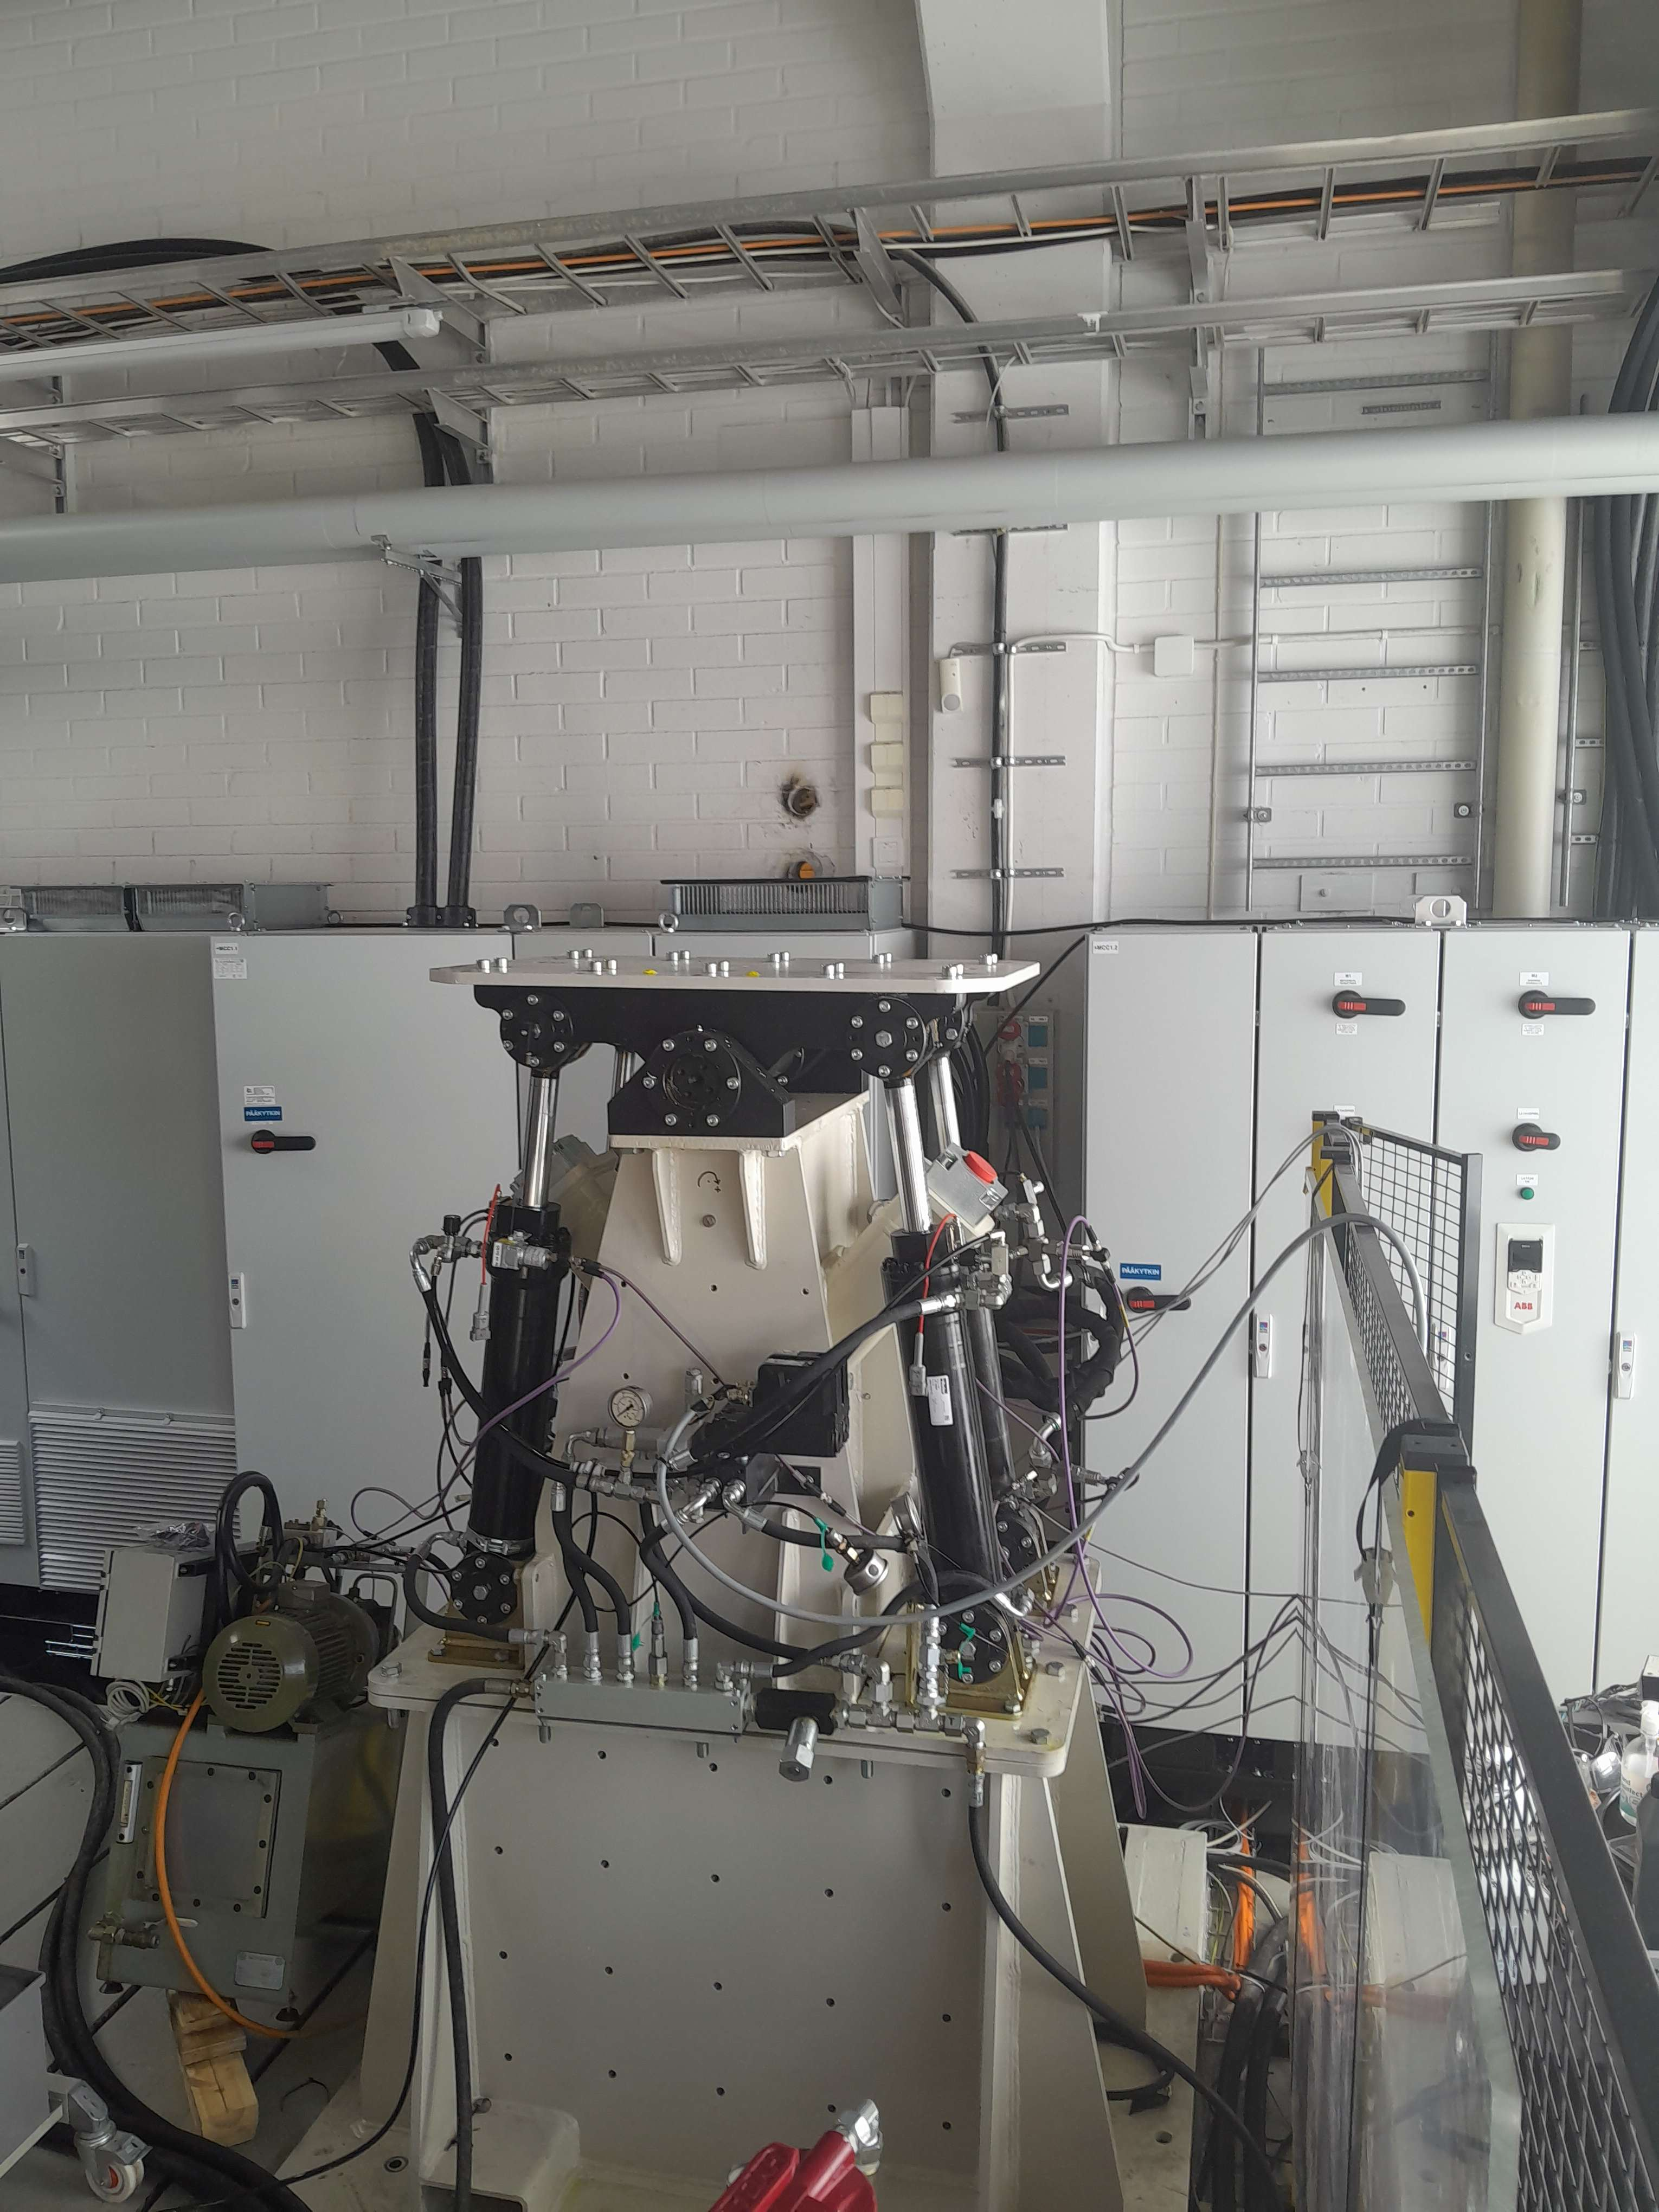
\includegraphics[width=0.4\textwidth]{assets/dolores}
	\caption{Dolores rotates the top platform about a pivot by actuating a pair of hydraulic cylinders.  A pair of additional cylinders in parallel can resist the motion providing loads useful for testing}\label{fig:dolores}
\end{figure}

The hydraulics are implemented as a DDH a.k.a. EHA system.  That kind of system was described by Zhang et al in~\cite{Zhang2017}.  The particular circuit is similar to that by Chiang in~\cite{Chiang2011}.

EHA/DDH was first noted in by~\cite{Helduser1995} in German, and he also did the first English-language publication in~\cite{Helduser1999}.

\subsubsection{Old System}

Prior to the work for this thesis, Dolores was controlled by Matlab and Simulink code wherein sensor readings were taken over a CAN bus through a USB-CAN dongle to the Simulink Vector CAN interface [cite].  The devices on the CAN bus were initialized using the Vector CANalyzer program.  The control program sent motor commands to a Parker ECU, seen in figure~\ref{fig:dolores_old_system}, over CANopen, which itself would send commands to the ABB inverter that drove the motor.  It also sent signals to a shuttle valve through a National Instruments DAQ, which was stepped up in power with a relay and a bench-top power supply.

\begin{figure}[h]
	\centering
	\includegraphics[width=0.4\textwidth]{assets/old_dolores_controls}
	\caption{The previous control system had an ECU (center), power supplies for valves (bottom), readouts for flows in the hydraulic circuit (top), and a cabinet containing the inverter for the electric motor (left).  Not depicted is the National Instruments DAQ and the CAN-USB dongle.}\label{fig:dolores_old_system}
\end{figure}

Pros:
\begin{enumerate}
	\item can be programmed with Matlab/Simulink (\textbf{FLEXIBLE})
	\item it worked
\end{enumerate}

Cons:
\begin{enumerate}
	\item components provided by 6 vendors (\textbf{SLOW})
	\item two components only for motor control (inverter, ECU), two components for IO (DAQ, CAN dongle) (\textbf{SLOW}, \textbf{GOOD})
	\item multiple programs running for initialization (\textbf{BAD}, \textbf{SLOW})
	\item every part of the system is opaque (\textbf{BAD})
	\item supporting new interfaces requires adding more components and thus complexity (\textbf{RIGID})
\end{enumerate}

\subsubsection{New System}

An industry collaborator on the GOOD project required that we use EtherCAT~\cite{Andreeva2023} to communicate with some inverters they were providing for the project.  This meant that the extant control hardware needed to be replaced with something that supports EtherCAT.

Additionally, a different industry partner suggested driving our hardware to run in tandem with software simulations, principally with the Mevea physics system~\cite{MeveaSoftware}.  Because of this, it was a priority to design the control systems that could integrate with external applications.  However, to date there haven't been any experiments that have called for this.  So while it was an important factor in the initial selection, external integrations haven't been thoroughly exercised.

It was also understood that the already-installed CAN-based sensors would remain in place, so CAN support was a requirement for the system.  With the benefit of hindsight, if this requirement were not there, commissioning these control systems would have been faster, but there was not the institutional knowledge in Aalto's Fluid Power Lab to anticipate this.

I considered two option in how to change the system.  One was to use a Speedgoat Realtime system and the other to use a PLC from Beckhoff Automation.  After studying both options, I implemented the control system with the Beckhoff PLC.  The reasoning for why follows.

The Speedgoat system was the first system I considered.  Behind the branding, these were regular computers which ran QNX, a UNIX-like, real-time operating system~\cite{SpeedgoatMachine, QnxSdp}.  It has an interface with Matlab and Simulink, and in fact, these interfaces are the intended principal means of administering these computers.

The principal benefit of this systems was its deep integration with Matlab and Simulink, which are familiar to the other researchers working on the GOOD project.  It would enable at least some degree of code reuse between simulation and hardware testing, which would speed up iteration time and so allow greater research output.

With respect to IO, Speedgoat sells expansions for CAN and digital IO like needed for valves.  They were fairly pricey and seemed as though they could not be easily used with non-Speedgoat systems, but they presumably worked in their intended context.  It's also possible for Speedgoat to communicate with 3rd-party IO devices over EtherCAT.  Since EtherCAT terminals from Beckhoff Automation are relatively cheap and staff in our lab had experience with them, we considered them a strong option.

Integration with external applications is where Speedgoat fell flat.  interfaces with external applications couldn't be used directly in the Simulink models since they run on the Speedgoat system and not the workstation which has the external applications.  The solution to this is to communicate over a local network information about the system state.  Speedgoat is able to use Simulink's network communication blocks to send messages over TCP/IP or UDP~\cite{SimulinkNetworkComms}.  However, I was not able to get reliable communication from reproducing the examples in the documentation.  Better was communication with the Matlab's Instrument Control Toolbox, but that can only (easily) be used to create virtual control panels in Matlab, not more general interfaces~\cite{SimulinkInstrument}.  There was also an option to use an open-source networking library like Zero MQ, but that would have required obtaining a C++ compiler compatible with QNX and then creating the Simulink blocks to access it, which would be difficult and expensive~\cite{ZeroMQ}.

I considered its strong guarantees of real-time performance, however, I never could find a case where they seemed to matter.  A real-time system is one where the low-level computer systems support running a program with a fixed time step, and often that time step is small and has little error.  Small time steps are nice, but Dolores is massive and has the large time constants associate with that, so very small time steps ($\mathcal{O}(\unit{\micro\second})$) won't provide any control benefit.  As well, I don't know that a time step coming late or early would disrupt control function, so I felt it appropriate to ignore this kind of timing jitter and allow issues related to it to be discovered instead of anticipated.  To date, this has caused no issues.

While its deep integration with Matlab and Simulink is appealing, the high difficulty in integrating with external tools made it an untenable choice.

The Beckhoff PLC was better, but not perfect.  Under the hood, they are regular computers that run Windows.  A PLC isn't a special type of computer, it just means that programs are written with computer languages specified by \mbox{IEC 61131-3}~\cite{IEC61131-3}.  For Beckhoff's systems, the development tools for these languages are provided by the TwinCAT IDE~\cite{BeckhoffTwinCAT}.  As mentioned previously, Beckhoff sells hardware for EtherCAT IO, and that includes a CAN master device~\cite{BeckhoffEL6751}.

It is a drawback that programs can't be written directly in Matlab or Simulink with the PLC hardware.  However, there was already some knowledge of the PLC language Structured Text in the lab and Beckhoff offers some products for interfacing with Matlab~\cite{BeckhoffMatlabInterface}.  So there was a possibility of using more familiar tools, though those interfaces received less support from Beckhoff than the native PLC code.  The PLC language for its part was fine.  It competently afforded moving data in and out of hardware and it had some facilities for abstracting low-level behaviors into higher-level concepts using Function Blocks, which are similar to classes in C++.

Through some informal experiments, I found the IO hardware and software to be reasonable to work with.  Program variables could be declared as an input or output and then linked with a register on the IO device.  To access these registers, the TwinCAT IDE could scan for all the devices available on the EtherCAT network and create a device tree containing IO registers and configuration data.  However, in time I would discover that doing this uncarefully could break the existing links which would take a long time to recreate.

\begin{figure}[h]
	\centering
	\includegraphics[width=0.4\textwidth]{assets/new_dolores_controls}
	\caption{foo}\label{fig:dolores_new_system}
\end{figure}

IO over CAN was much more difficult.  While Beckhoff officially supports it, the available documentation is sparse, difficult to find, and doesn't include critical configuration procedures.  The only way to learn these things is to contact support.  This can take a long time, since to the best of my knowledge, Beckhoff has only one support person knowledgeable in the CAN system in Finland.  Even after getting support, major features like initialization were missing and needed to be provided with the Vector CAN tools used in the old system.  From notes in unrelated documentation I could find, it appears that initialization at least is technically implemented, but the means to enable it remain elusive.

The inverter which was provided, an ABB ACS880, can be commanded with the CiA 402 protocol~\cite{ACS880, CiA402}.  It would appear that TwinCAT has built-in support for this protocol, however it appears that it's locked behind using their motor control products, e.g. EP7211~\cite{EP7211}.  While it would have been desirable to do so, this project was constrained by industry collaborators to communicate with the inverters directly over EtherCAT.  Therefore it was necessary to create a new implementation of this protocol which doesn't demand other hardware.  This wasn't extremely difficult; the protocol just describes a finite state machine to bring the drive into an operational state.  However, without any facilities for error handling, like \verb|try|/\verb|catch| blocks in C++~\cite{CppTryCatch} or \verb|Result|s in Rust~\cite{RustResult}, it was very tricky to implement error handling and I am not confident that the current implementation is completely reliable.  This means that the drive can potentially enter an unsafe fault state which would need to be handled by a human operator hitting an emergency stop switch.

All these IO cards came with long lead times for orders, sometimes up to months.  Beckhoff claims this is due to supply chain issues stemming from the past years of social and political upheaval around the world.  Regardless, I doubt Speedgoat delivers much faster given they are a much smaller vendor.

Interfacing with external programs was possible through a built-in network UDP interface~\cite{BeckhoffTcpUdpRealtime}.  It requires configuration and about 150 lines of code to create the server on the PLC side.  Then the external application can communicate with it as though it's like any other UDP server on the internet.  An example I created of how this is implemented can be found online in~\cite{PorterGoodPlc}.  The PLC portion found at the path \verb|/good_system/Dolores/POUs/Server.TcPOU| and the external application at \verb|/plc_client/plc_client.py|.  TwinCAT's UDP API was sufficient to create a simple network interface for the PLC program, however when I tried to create more complex interfaces, it frequently crashed and behind only cryptic, unhelpful error messages, if anything at all.

\subsection{A Novel Stack for a Pneumatic Stewart Platform}

With this new theory of a mechatronic tech stack, it made sense to start a project to study what tools this model lends itself to when applied prescriptively.  The project was a driving simulator chair that had been an unfinished student project a year prior~\cite{Bjoerklund2023}.  The mechanical systems had been finished including all the sensors and transducers, so all that was needed was a control system.

The system is a chair atop a stewart platform whose linear actuators are single-acting pneumatic-muscle cylinders~\cite{Stewart1965, Caldwell1995}.  The valve manifolds that were already made for this had one valve to connect the pneumatic muscle to an external pressure source and another to vent the muscle to atmosphere.  If both valves were closed, it would brake the cylinder.  It was avoided to open both since it would vent the pressure source to atmosphere.  There are 6 instances of this circuit, connected to the common pressure source in series.  Each cylinder also has a position sensor, which exposes itself as a voltage signal from a potentiometer.

Tool selection started from the bottom of the stack, namely IO.\  The need was to switch 12 digital outputs for the valves, each about $\qty{2}{\watt}$, and six analog inputs ($\qtyrange[range-units=single,range-phrase=..]{0}{24}{\volt}$) from the position sensors.  It was also desirable for the work to be done quickly to have a demonstration in time for publication.  This was met with EtherCAT IO cards from Beckhoff~GmbH, in large part thanks to their availability within our lab.  They supply digital output cards and analog input cards that mostly met the requirements; the digital ouputs needed to be supplemented with flyback diodes due to the inductive load and the analog inputs needed signals stepped down to $\qtyrange[range-units=single,range-phrase=..]{0}{10}{\volt}$ with resistors~\cite{BeckhoffEL2042,BeckhoffEL3062}.  This meant routing signal cables from the sensors and transducers to terminal blocks, placing the diodes and resistors in the terminals, and from there on to the Beckhoff terminals.  There then is an EtherCAT connection from the block of Beckhoff terminals to the computer's Ethernet port~\cite{BeckhoffEK1100}.

In selecting the computer, it needed to communicate with the IO over EtherCAT and be cheap and easy to develop for.  The Raspberry Pi supports EtherCAT, was only 54€ ($\approx$¥9000), and for us working on the project, the Linux-based systems are familiar and easy to use.

The principle middleware requirement was an EtherCAT master, which itself depends on system-level networking, that then may have its own dependencies.  By using Linux, all of those requirements except for the EtherCAT master are met.  Conventionally, PLC-based systems, like those from Beckhoff, are used for EtherCAT masters~\cite{BeckhoffTwinCAT}.  However, those generally do not run on Linux.  However, part of the point of this project was to try new things.  So, Ethercrab, which is a master written in the Rust programming language, was used~\cite{Ethercrab}.  Ethercrab benefits from being open source, so motivated users can troubleshoot more easily.  It also has thorough documentation with lots of examples (see e.g.\ \verb|ethercrab/examples/ek1100.rs|).  It is also a Rust library and Rust is an increasingly popular programming language on account of it's ease of making changes to code, quality tooling, performance, and memory safety~\cite{RustHomePage}.

CONTROL LAYER

\subsection{A Recorder-Playing Robot}

Gonna cite Masuda-san~\cite{Masuda2012}

\lipsum[1-3]

\clearpage


\section{Results and Discussion}

\lipsum[1-3]

\subsection{Future Work}

\lipsum[8-9]

\clearpage


\section{Conclusion}

\lipsum[1-4]

\clearpage

\phantomsection
\addcontentsline{toc}{section}{\refname}
%%\addcontentsline{toc}{section}{References}

\bibliographystyle{ieeetr}
\bibliography{bib/good-masters.bib}

%% Appendices
%% Liitteet
\clearpage

\thesisappendix

% Appendix

\end{document}
